\chapter{Angular}
Para crear un nuevo proyecto ejecutamos en un cmd en modo administrador :\\
\texttt{ng new nombreProyecto}\\
Elegimos N y  con CSS como se muestra en la figura.\\
\begin{figure}[H] % Ambiente 'figure'
	\centering % imagen sin escalar
	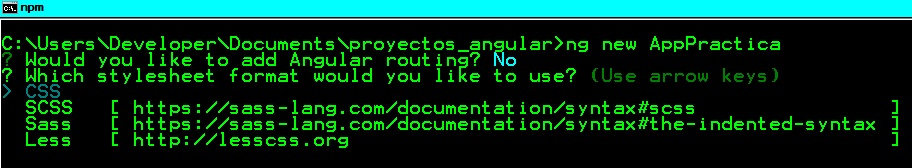
\includegraphics[scale=0.6]{images/c3_1.jpg}
	\caption{Creando proyecto angular.}
\end{figure}
Para levantar servidor local.Nos ubicamos  a nivel de la ruta del proyecto creado y levantamos el servidor local.\\
\texttt{ng serve -o}\\
\begin{figure}[H] % Ambiente 'figure'
	\centering % imagen sin escalar
	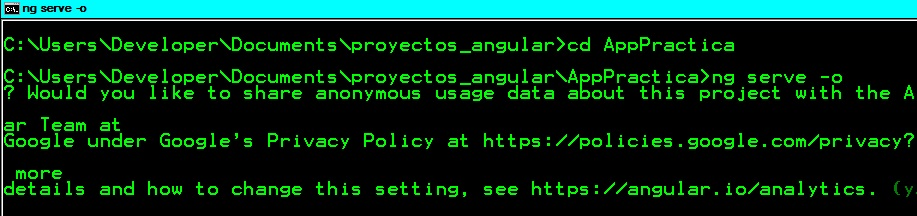
\includegraphics[scale=0.6]{images/c3_2.jpg}
	\caption{Servidor local angular.}
\end{figure}
En el navegador web mediante el siguiente url podemos ver el proyecto levantado localmente.\\
\url{http://localhost:4200/}\\


\section{Estructura del proyecto.}
La estructura esta ordenada de tal manera que es entendible a simple vista .Entre los directorios
principales tenemos :
\begin{itemize}
	\item e2e:Es para correr las pruebas automaticas,unitarias e iintegraci\'on.
	\item node\_modules:Tiene las dependencias externas instaladas con el comando npm.
	Como librer\'\i{}as graficas,uso de calendarios,\\encriptaci\'on,etc.
	\item Src: Se encuentra el c\'odigo fuente de la app ,los componentes y p\'aginas.
	\item tsconfig.json: Configuraciones para TypeScript.
	\item tslint.json: Se encuentran las reglas para JavaScript y TypeScript.
\end{itemize}
\begin{figure}[H] % Ambiente 'figure'
	\centering % imagen sin escalar
	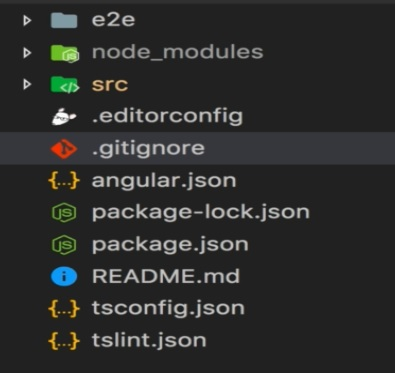
\includegraphics[scale=0.7]{images/c3_4.jpg}
	\caption{Estructura del proyecto.}
\end{figure}
Para crear un componente en angular se ejecuta el siguiente comando :\\
 \texttt{ng g c components/footer}\\

\section{Bootstrap mediante Angular Cli.}
De manera local instalaremos mediante angular cli las siguientes librerias.\\
 \texttt{npm install bootstrap --save}\\
 \texttt{npm install jquery --save}\\
 \texttt{npm install popper.js --save}\\
 En angular.json , ponemos las rutas de los styles y scripts,anteriormente instalados.
 \begin{figure}[H] % Ambiente 'figure'
 	\centering % imagen sin escalar
 	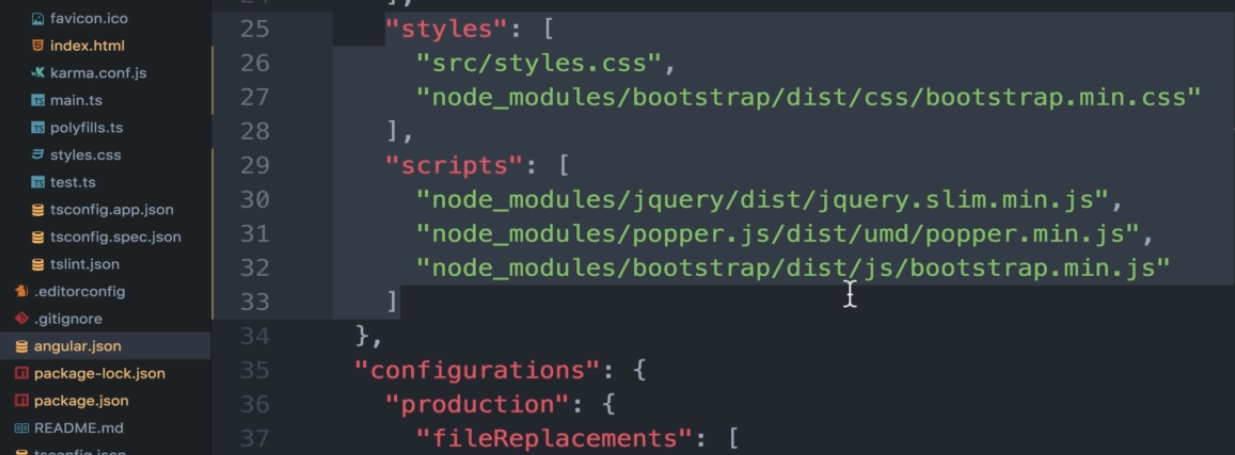
\includegraphics[scale=0.5]{images/c3_5.jpg}
 	\caption{El archivo angular.json.}
 \end{figure}

\section{Angular en produccion.}
Instalaremos un server de pruebas de preproduccion de node.\\
 \texttt{npm install http-server -g}\\
 Ahora generaremos los archivos para probar en ese servidor.\\
Los resultados estan en la carpeta dist\\
 \texttt{ng build}\\
  En la carpeta dist, dentro se crea una carpeta.Nos ubicamos en esa carpeta y  ejecutamos.\\
 \texttt{http-server -o}\\
 \subsection{ Produccion.}
 Generando archivos para produccion.Borrar  la
 carpeta dist.\\Los resultados estan en la carpeta dist\\
 \texttt{ng build --prod}\\
 Nos ubicamos en la ruta dist/carpetaGenerada.Como se muestra de ejemplo.\\
  \texttt{ cd C:Users\textbackslash{}Developer\textbackslash{}Documents\textbackslash{}AngularProyectos\textbackslash{}AppGeneral\textbackslash{}dist\textbackslash{}AppGeneral}\\
  \texttt{http-server -o}\\
  Este servidor es de pre produccion.Una vez ya probado todo hacemos el despliegue en el servidor de produccion real.\\Subimos la carpeta de la app que esta en la carpeta  dist.\\
   \subsection{ Solucion a recarga de pagina web en produccion.}
   La pagina web no recarga,esto se soluciona agrgando en nuestro proyecto en el archivo app.routes.ts
   la siguiente instruccion como se muestra en la figura.
\begin{figure}[H] % Ambiente 'figure'
	\centering % imagen sin escalar
	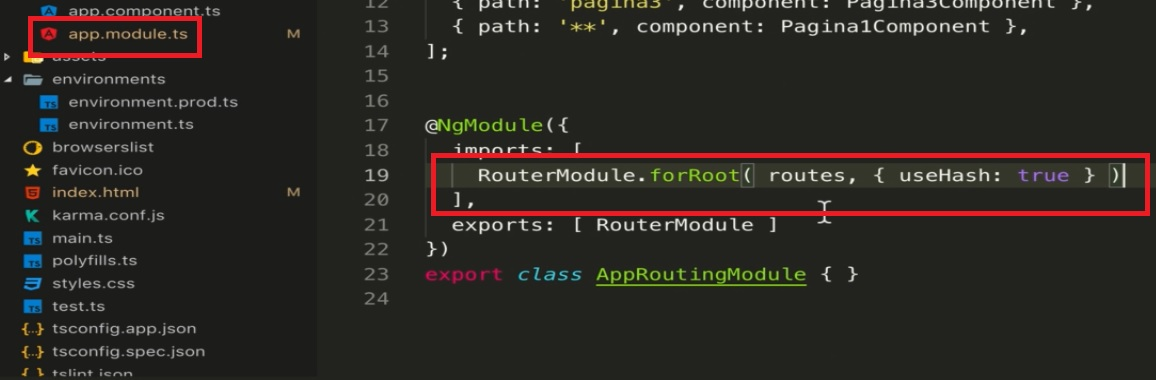
\includegraphics[scale=0.55]{images/c3_6.jpg}
	\caption{Solucion a recarga de pagina.}
\end{figure}
 \subsection{ Solucion a recurso no encontrado de pagina web en produccion.}
 Se debe corregir la ruta que se hace referencia, en el archivo index.html agregando la siguiente instruccion que se muestra en la figura.
 \begin{figure}[H] % Ambiente 'figure'
 	\centering % imagen sin escalar
 	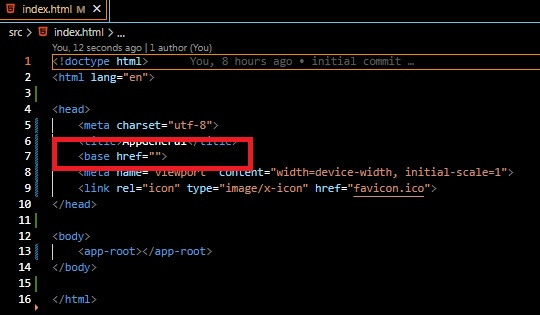
\includegraphics[scale=1.2]{images/c3_7.jpg}
 	\caption{Solucion a recurso que no carga de pagina web.}
 \end{figure}







